\part*{Principles of Computer Organization}
\pdfbookmark[1]{Principles of Computer Organization}{Principles of Computer Organization}

The principles of computer system, the most basic knowledges of computer science.

\section*{1 Overview of Computer Sysetm}
\pdfbookmark[2]{1 Overview of Computer System}{overview of computer system}

\subsection*{1.1 Composition of computer system}

\begin{flushleft}
	\colorbox{yellow}{Computer System = Hardware + Software}

	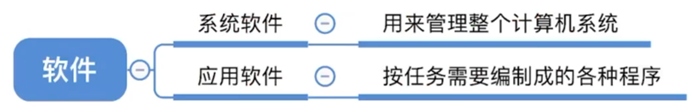
\includegraphics{images/principles_of_computer_organization/softwares}

	System softwares: operating system, DBMS, standard libraries, compiler, etc.

	Application softwares: video games, office tools, chat tools, etc.
\end{flushleft}

\subsection*{1.2 The development of computer}

\begin{flushleft}
        The history of development

        \begin{itemize}
            \item the Era of electron tube
		    \begin{itemize}
			\item use the electron tube
			\item very large volume and power consumption
        	    \end{itemize}
    	    \item the Era of Transistor tube
                    \begin{itemize}
		        \item use the transistor tube
		        \item the volume is greatly reduced, and there is a qualitative leap on the calculation speed
		        \item high-level programming languages begin to appear, and operating system begins to take shape
                    \end{itemize}
            \item the Era of small and  medium scale integrated circuits
        	    \begin{itemize}
		        \item integrate the components on a substrate
		        \item the reliability is enhanced to a large extent
		        \item high-level programming languages are developing rapidly 
	            \end{itemize}
            \item the Era of VLSI
                    \begin{itemize}
		        \item microprocessor and microcomputer begin to appear
		        \item personal computer begins to popularize
		        \item modern operating systems, such as Windows, MacOS and Linux, are born
                    \end{itemize}
        \end{itemize}

	The development trend

        \begin{itemize}
		\item Microcomputer
		\item Supercomputer
        \end{itemize}
\end{flushleft}

\subsection*{1.3 Composition of computer hardware}

\newpage

\section*{2 Representation and operation of data in computer}
\pdfbookmark[2]{2 Representation and operation of data in computer}{Representation and operation of data in computer}

\subsection*{2.1 the round-counting system}

\begin{flushleft}

	Reasons for using binary

	\begin{itemize}
		\item It can be represented by a physical device with two steady states, which is low cost and easy to implement.
		\item 0 and 1 exactly correspond to the false and true values of logical values, making it convenient to implement logical operations.
		\item It is convenient to use logic gate circuits to perform arithmetic operations.
	\end{itemize}

	Convert an r-base number to a decimal number
	
	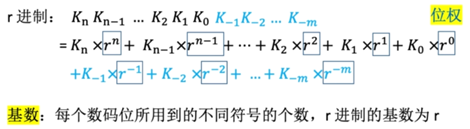
\includegraphics{images/principles_of_computer_organization/r-base_to_decimal}

	Conversion between octal and hexadecimal

	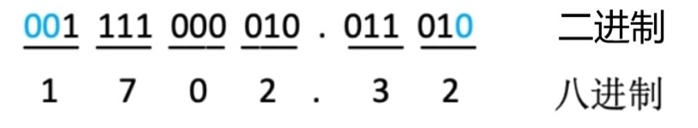
\includegraphics{images/principles_of_computer_organization/binary_octal}
	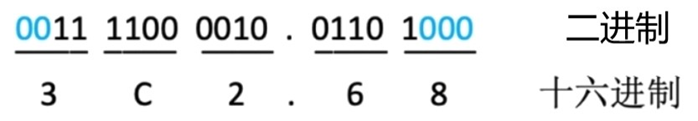
\includegraphics{images/principles_of_computer_organization/binary_hexadecimal}

\end{flushleft}

\subsection*{2.2 the representation and operation of unsigned number}

\newpage

\section*{3 Storage System}
\pdfbookmark[2]{3 Storage System}{Storage System}

\newpage

\section*{4 Instruct System}  
\pdfbookmark[2]{4 Instruct System}{Instruct System}

\newpage

\section*{5 Central Processor Unit}  
\pdfbookmark[2]{5 Central Processor Unit}{Central Processor Unit}

\newpage

\section*{6 Bus}  
\pdfbookmark[2]{6 Bus}{Bus}

\newpage

\section*{7 I/O System}  
\pdfbookmark[2]{7 I/O System}{I/O System}
